\section{Projektion auf die Eigengesichter} \label{sec:eigenbasis}
\begin{tcolorbox}
	\centerline{\textbf{Lernziele Kapitel~\ref{sec:eigenbasis}}}
	\begin{enumerate}[leftmargin=*,label=\thesection.\arabic*]
		\item \label{item:projection} Die Lernenden können die Projektion eines Vektors auf einen Unterraum berechnen, wenn eine orthonormale Basis dieses Unterraumes gegeben ist.\\
		(Aufgaben~\ref{aufg:projection_3d} und~\ref{aufg:projection})
		\item \label{item:compute_coefficients} Die Lernenden können das Skalarprodukt von Vektoren in Python berechnen.\\
		(Aufgabe~\ref{aufg:compute_coefficients})
	\end{enumerate}
\end{tcolorbox}
In diesem Unterkapitel wollen wir allgemeine Bilder als Linearkombination der Eigengesichter darstellen.
Man kann zeigen, dass alle Bilder der Datenbank exakt als Linearkombination der Eigengesichter geschrieben werden können.
Neue Bilder können im Allgemeinen mit so einer Linearkombination nur angenähert werden.
Die beste Näherung ist gerade die Projektion des neuen Bildes auf den Raum, der durch die Eigengesichter aufgespannt wird.
Was das genau bedeutet, wollen wir zuerst im drei Dimensionen veranschaulichen.
\begin{figure}[ht]
	\centering
	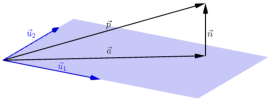
\includegraphics[width=0.5\textwidth]{images/projection}
	\caption{Projektion $\vec a$ von $\vec p$ auf die Ebene durch Null, die von $\vec v_1$ und $\vec v_2$ aufgespannt wird. Der Vektor $\vec n$ steht normal auf die Ebene und es gilt $\vec p=\vec a+\vec n$.}
	\label{fig:projection}
\end{figure}
\begin{aufgabe} \label{aufg:projection_3d}
	Betrachten Sie die Vektoren
	\begin{equation*}
		\vec v_1=\frac{1}{\sqrt{3}}\begin{pmatrix}
			1 \\ 1 \\ 1
		\end{pmatrix},\quad
		\vec v_2=\frac{1}{\sqrt{2}}\begin{pmatrix}
			-1 \\ 1 \\  0
		\end{pmatrix},\quad
		\vec p=\begin{pmatrix}
			3 \\ 1 \\  2
		\end{pmatrix}.
	\end{equation*}
	\begin{enumerate}[label=(\alph*)]
		\item Sind die Vektoren $\vec v_1$ und $\vec v_2$ orthonormal? Begründen Sie.
		\item Die Vektoren $\vec v_1$ und $\vec v_2$ spannen eine Ebene durch den Nullpunkt auf.
		Berechnen Sie den Vektor $\vec a$, welcher der orthogonalen Projektion von $\vec p$ auf diese Ebene entspricht.
		Dazu können Sie zum Beispiel eine Zerlegung $\vec p=\vec a+\vec n$ wie in Abbildung~\ref{fig:projection} machen.
		\item Dann kann man $\vec a$ als Linearkombination vom $\vec v_1$ und $\vec v_2$ darstellen, also
		\begin{equation*}
			\vec a=c_1\vec v_1+c_2\vec v_2.
		\end{equation*}
		Berechnen Sie die Koeffizienten $c_1$ und $c_2$ in Termen von $\vec v_1,\vec v_2$ und $\vec p$.
	\end{enumerate}
\end{aufgabe}
\begin{losung}
	\begin{enumerate}[label=(\alph*)]
		\item Die Vektoren sind orthogonal, denn ihr Skalarprodukt ist Null
		\begin{equation*}
			\vec v_1\cdot\vec v_2= \frac{1}{\sqrt{3}}\cdot\frac{1}{\sqrt{2}}\cdot\left(1\cdot\left(-1\right)+1\cdot 1+1\cdot 0\right)=0.
		\end{equation*}
		Sie sind sogar orthonormal, denn sie haben auch Länge 1, weil
		\begin{equation*}
			\vec v_1\cdot\vec v_1=\frac{1}{3}\left(1^2+1^2+1^2\right)=1
		\end{equation*}
		und
		\begin{equation*}
			\vec v_2\cdot\vec v_2=\frac{1}{2}\left(\left(-1\right)^2+1^2+0^2\right)=1.
		\end{equation*}
		\item Wir zerlegen $\vec p=\vec a+\vec n$ wie in Abbildung~\ref{fig:projection} in einen Vektor $\vec a$ der in der Ebene liegt und einen Vektor $\vec n$ der orthogonal zur Ebene steht.
		Gesucht ist der Vektor $\vec a$.
		Da er in der Ebene liegt, gibt es eindeutige Koeffizienten $c_1$ und $c_2$, so dass
		\begin{equation*}
			\vec a=c_1\vec v_1+c_2\vec v_2.
		\end{equation*}
		Wir addieren $\vec n$ auf beiden Seiten und erhalten
		\begin{equation*}
			\vec p=c_1\vec v_1+c_2\vec v_2+\vec n.
		\end{equation*}
		Nun bilden wir auf beiden Seiten das Skalarprodukt mit $\vec v_1$, also
		\begin{equation*}
			\vec v_1\cdot\vec p=c_1\underbrace{\vec v_1\cdot\vec v_1}_{=1}+c_2\underbrace{\vec v_1\cdot\vec v_2}_{=0}+\underbrace{\vec v_1\cdot\vec n}_{=0}.
		\end{equation*}
		Hier haben wir verwendet, dass $\vec v_1$ orthogonal ist zu $\vec v_2$ und $\vec n$.
		Wir erhalten
		\begin{equation*}
			c_1=\vec v_1\cdot\vec p=\frac{6}{\sqrt{3}}.
		\end{equation*}
		In dem man stattdessen auf beiden Seiten das Skalarprodukt mit $\vec v_2$ bildet, erhält man analog
		\begin{equation*}
			c_2=\vec v_2\cdot\vec p=-\frac{2}{\sqrt{2}}.
		\end{equation*}
		Damit berechnen wir die Projektion
		\begin{equation*}
			\vec a
			=c_1\vec v_1+c_2\vec v_2
			=2\begin{pmatrix}
				1 \\ 1 \\ 1
			\end{pmatrix}
			-2\begin{pmatrix}
				-1 \\ 1 \\ 0
			\end{pmatrix}
			=\begin{pmatrix}
				4 \\ 0 \\ 2
			\end{pmatrix}.
		\end{equation*}
		\item In der Lösung der vorherigen Teilaufgabe haben wir die Koeffizienten schon berechnet zu
		\begin{equation*}
			c_1=\frac{6}{\sqrt{3}}
			\quad\quad\text{und}\quad\quad
			c_2=-\frac{2}{\sqrt{2}}.
		\end{equation*}
	\end{enumerate}
\end{losung}

Was wir in der vorherigen Teilaufgabe berechnet haben, funktioniert auch in höheren Dimensionen.
Die Vektoren $\vec v,\vec w$ und $\vec p$ sollen nun jeweils $M\cdot N$ Komponenten haben.
Wir sagen, die zwei Vektoren sind orthogonal, wenn $\vec v\cdot\vec w=0$.
Falls sie zusätzlich Länge 1 haben, also $\vec v\cdot\vec v=1$ und $\vec w\cdot\vec w=1$, dann heissen sie orthonormal.
Eine Familie $\vec v_1,\ldots,\vec v_K$ heisst orthonormal, wenn die Vektoren alle paarweise orthonormal sind.
Sie spannen dann einen $K$-dimensionalen Raum auf.
Wir können wie in Aufgabe~\ref{aufg:projection_3d} die Projektion des Vektors $\vec p$ auf diesen Raum berechnen, nämlich
\begin{equation*}
	c_1\vec v_1+\ldots+c_K\vec v_K,
\end{equation*}
wobei die Koeffizienten gegeben sind durch
\begin{equation*}
	c_k=\vec v_k\cdot\vec p,\qquad k=1,\ldots,K.
\end{equation*}
Nun betrachten wir wieder die Eigengesichter $\vec u_1,\ldots,\vec u_K$.
Gemäss der Konstruktion aus dem letzten Kapitel sind diese orthonormal.
Wir betrachten zudem die Mona Lisa von Leonardo da Vinci, ein Bild das nicht in unserer Datenbank ist.
Den entsprechenden Vektor nennen wir $\vec p$.
Um dieses Bild in den Raum zu verschieben, der von den Differenzgesichtern (oder von den Eigengesichtern) aufgespannt wird, müssen wir noch das Durchschnittsgesicht $\vec m$ subtrahieren.
Das entstehende Differenzgesicht kann dann näherungsweise als Linearkombination der Differenzgesichter $\vec a_1,\ldots,\vec a_K$ oder auch der Eigengesichter $\vec u_1,\ldots,\vec u_K$ dargestellt werden (diese spannen den selben Raum auf).
Nur näherungsweise deswegen, weil wir lediglich eine Projektion auf den Raum der Differenzgesichter (oder Eigengesichter) berechnen.
Das Differenzgesicht des neuen Gesichtes liegt aber nicht notwendigerweise in diesem Raum.
Diese Projektion berechnet sich wie oben beschrieben.
\begin{aufgabe} \label{aufg:projection}
	Sei $\vec p$ das Bild der Mona Lisa und $\vec u_1,\ldots,\vec u_K$ die Eigengesichter.
	Berechnen Sie die Koeffizienten $c_1,\ldots,c_K$ der Projektion von $\vec p-\vec m$ auf die Eigengesichter.
	Geben Sie die Koeffizienten in Termen von $\vec p,\vec m$ und den Eigengesichtern an.
\end{aufgabe}
\begin{losung}
	Wir verfahren analog zu Aufgabe~\ref{aufg:projection_3d}, nur das wir jetzt nicht $\vec{p}$, sondern $\vec p-\vec m$ projizieren müssen.
	Das heisst, wir teilen diesen Vektor auf in eine noch unbekannte Linearkombination der Eigengesichter und einen dazu orthogonalen Teil $\vec{n}$, also
	\begin{equation*}
		\vec p-\vec m=c_1\vec u_1+c_2\vec u_2+\ldots+c_K\vec u_K+\vec{n}.
	\end{equation*}
	Wir bilden das Skalarprodukt beider Seiten der obigen Gleichung mit $u_1$, also
	\begin{equation*}
		\vec u_1\cdot\left(\vec p-\vec m\right)=c_1\underbrace{\vec u_1\cdot\vec u_1}_{=1}+c_2\underbrace{\vec u_1\cdot\vec u_2}_{=0}+\ldots+c_K\underbrace{\vec u_1\cdot\vec u_K}_{=0}.
	\end{equation*}
	Weil die Eigengesichter orthonormal sind, vereinfacht sich das zu
	\begin{equation*}
		\vec u_1\cdot\left(\vec p-\vec m\right)=c_1.
	\end{equation*}
	Wenn wir das auch noch mit $\vec u_2,\ldots,\vec u_K$ machen erhalten wir
	\begin{equation*}
		\vec u_k\cdot\left(\vec p-\vec m\right)=c_k,
	\end{equation*}
	für alle $k\in\{1,\ldots,K\}$.
\end{losung}

Hat man die Koeffizienten der Linearkombination berechnet, so kann die Projektion der Mona Lisa wieder als Linearkombination der Eigengesichter und des Durchschnittsgesichtes darstellen
\begin{equation*}
	\vec m+c_1\vec u_1+c_2\vec u_2+\ldots+c_Ku_K.
\end{equation*}
\begin{aufgabe} \label{aufg:compute_coefficients}
	Seien \texttt{p} und \texttt{m} Vektoren mit $M\cdot N$ Komponenten, wobei \texttt{p} ein Gesicht zeigt (z.B. das der Mona Lisa) und \texttt{m} das Durchschnittsgesicht ist.
	Sei zudem \texttt{u\_list} die Liste der Eigengesichter.
	Ergänzen Sie die Funktion \texttt{compute\_coefficients(p, m, u\_list)}, welche die Liste der Koeffizienten der Linearkombination aus Abbildung~\ref{fig:eigen_basis} zurück gibt.
	Um Ihre Lösung zu testen können Sie das Python Skript \texttt{basis\_expansion.py} laufen lassen, welches die Projektion der Mona Lisa mit den von Ihnen berechneten Koeffizienten darstellt.
	\textit{Hinweis:} Mit \texttt{np.dot(v,w)} lässt sich das Skalarprodukt zweier Vektoren \texttt{v} und \texttt{w} berechnen.
\end{aufgabe}
\begin{losung}
	Die Lösung könnte zum Beispiel so aussehen.\\[0.5cm]
	\begin{minipage}{0.65\textwidth}
\begin{lstlisting}[style=python]
import numpy as np

def compute_coefficients(p, m, u_list):
	K = len(u_list)
	c_list = np.empty((K,))
	for k in range(K):
		c[k] = np.dot(u[k], p - m)
	return c_list
\end{lstlisting}
	\end{minipage}\hfill
	\begin{minipage}{0.35\textwidth}\vspace{-1cm}
		\centering Rekonstruktion:\\[0.5cm]
		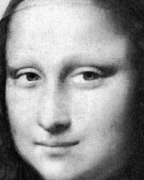
\includegraphics[width=0.4\textwidth]{images/eigenfaces/mona_lisa_eigen_approx}
	\end{minipage}
\end{losung}

Anscheinend sieht die Projektion fast gleich aus wie das Bild selber.
Etwas informell ist das in in Abbildung~\ref{fig:eigen_basis} dargestellt.
Dieses Phänomen bedeutet, dass das Differenzgesicht der Mona Lisa ganz oder in sehr guter Näherung im Raum liegt, er durch die Eigengesichter aufgespannt wird.
%In Abbildung~\ref{fig:projection} würde das einem Vektor $\vec p-\vec m$ entsprechen, der mit der Ebene einen verschwindend kleinen Winkel einschliesst, also fast in der Ebene liegt.
Mit dieser Beobachtung wollen wir uns im nächsten Kapitel genauer auseinandersetzen.
\begin{figure}[ht]
	\centering
	\begin{tabular}{m{1.3cm} c c m{1.3cm} c c m{1.3cm} c c m{1.3cm} c c}
		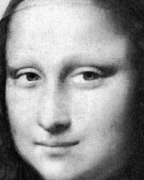
\includegraphics[width=0.08\textwidth]{images/eigenfaces/mona_lisa_eigen_approx} &
		$=$ & $0.17\ldots$ & 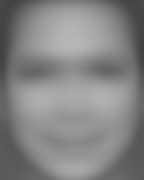
\includegraphics[width=0.08\textwidth]{images/facespace/meanface} & $+$ & $0.22\ldots$ & 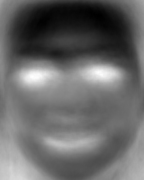
\includegraphics[width=0.08\textwidth]{images/eigenfaces/eigenface00}
		& $+$ & $0.10\ldots$ & 
\includegraphics[width=0.08\textwidth]{images/eigenfaces/eigenface01} & $+$ & $\cdots$
	\end{tabular}
	\caption{Die Projektion der Mona Lisa auf die Eigengesichter entspricht einer Überlagerung (Linearkombination) der Eigengesichter und des Durchschnittsgesichtes. Die Vorfaktoren sind nur symbolisch und entsprechen nicht den echten Werten.}
	\label{fig:eigen_basis}
\end{figure}